\subsection{Getting speedJ to work}
SpeedJ changes the speeds the every joint down the kinematic chain. This means we get a more flowing motion, however it comes at a cost. - Precision. 
\newline We have to update at the precise time to fit the speeds.
\newline A way of illustrating this would be Eulers method to first order differential equations. 
\newline Here everything is a little off as we always approximate with the tangent. This will get more and more off the real target the larger steps you take. 
\newline The same is true for this. This is actually really much the same.\newline

Another problem we will show is that we do not reach the targets we want to by using servoJ or moveL. there is an offset. Note that we are giving it a point it should be and reading out where it arrived at.
\newline This could mean that it takes in some offset to counterbalance the its own weight. However i do not know this. This is just me thinking.\newline

For the sake of reducing the text, i will only show the first and the last step in the record. For the full record i will give the path to the test.
\newline All of the tests is in radians. TimeStep is in seconds.
\newline These tests are done in simulation only if nothing else is noted.
\subsubsection{Raw speedJ with servoJ to get to startpoint}
Here we are trying to take a look at the problem. 
\newline As you can see. We are starting off. And even though these test are done precisely same, they start in different points. properly because of the wobble. We are waiting 3 seconds here to reduce wobble.
\newline Also the servoJ has some offset. 
\newline Here we are using servoJ to position us to the first point and using speedJ from there:

\paragraph{test1}
Full test at "tests/throwCalculationsTests/speedJTests/Test1.txt"\newline

start of test:\newline

throwPositions with timeStep:  0.05
\newline new throwPositions is a vector X: 41 Y:  6
\newline new recoveryPositions is a vector X: 21 Y:  6
\newline Thread priority is: Time Critical
\newline [0.000000s - Step 0/41]:
\newline \hspace{1cm}        pos(-1.313193, -1.579761, -1.450452, -0.220422, 1.501750, -0.064856) should be:
\newline \hspace{1cm}        pos(-1.178097, -1.570796, -1.265364, -0.087266, 1.483530, 0.000000)
\newline [2.000000s - Step 40/41]:
\newline \hspace{1cm}        pos(-1.447671, -1.822501, -1.549878, -1.323733, 1.550060, -0.258894) should be:
\newline \hspace{1cm}        pos(-1.379977, -1.871966, -1.389736, -1.450072, 1.569761, -0.203377)\newline

end of test.\newline

As you can see if we are not even hitting the position in servoJ. It is also noted that the robot stands and wobbles.\newline

positon error in the begging is pos(-0.135096, -0.008965, -0.185088, -0.136954, 0.01822, -0.064856)
\newline positon error in the end is pos(-0.067694, -0.049465, -0.160042, 0.126339, -0.019701, -0.055517)\newline 

\paragraph{test2}
Full test at "tests/throwCalculationsTests/speedJTests/Test2.txt"\newline

start of test:\newline

throwPositions with timeStep:  0.05
\newline new throwPositions is a vector X: 41 Y:  6
\newline new recoveryPositions is a vector X: 21 Y:  6
\newline Thread priority is: Time Critical
\newline [0.000000s - Step 0/41]:
\newline \hspace{1cm}        pos(-1.307165, -1.579367, -1.442189, -0.214486, 1.500933, -0.061969) should be:
\newline \hspace{1cm}        pos(-1.178097, -1.570796, -1.265364, -0.087266, 1.483530, 0.000000)
\newline [2.000000s - Step 40/41]:
\newline \hspace{1cm}        pos(-1.442427, -1.816584, -1.539463, -1.292029, 1.551028, -0.247493) should be:
\newline \hspace{1cm}       pos(-1.379977, -1.871966, -1.389736, -1.450072, 1.569761, -0.203377)\newline

end of test.\newline 

As you can see if we are not even hitting the position in servoJ. It is also noted that the robot stands and wobbles.\newline

positon error in the begging is pos(-0.129068, -0.008571, -0.176825, -0.127220, 0.017403, -0.061969)
\newline positon error in the end is pos(-0.062450, 0.055382, -0.149727, 0.158043, -0.018733, -0.044116)

\paragraph{Notes from tests}
As you can see there is a difference in start position of the two tests. The difference is pos(-0.006028, -0.000394, -0.008263, -0.009734, 0.000817, -0.002887), which is just weird. But small enough to be negligible.
\newline Also you can see there is a very big difference in where we want to be in the begging and where we end up. Note that this in radians and a very small step means a whole lot.\newline

converted to degrees, you can clearly see the picture:
\newline test 1 start: pos(-7.740431, -0.513657, -10.604761, -7.846886, 1.043929, -3.715975) degrees.
\newline test 2 start: pos(-7.395052, -0.491082, -10.131326, -7.289169, 0.997118, -3.550562) degrees.\newline 

This is really alot and is NOT negligible.

The average of these two start positions is pos(-1.310179, -1.579564, -1.446321, -0.217454, 1.501342, -0.063413). \newline 
The error from this is pos(-0.132082, -0.008768, -0.180957, -0.130188, 0.017812, -0.063413).
\newline We will use this in the next tests.

\subsubsection{Raw speedJ with TM to get to startpoint and a moveL}
To get a clearer picture of why we are so much off in start position from where we want to be, we will try using a craigs DH parameters and generating a TM and converting to UR axis angles and use moveL to position us.

\paragraph{test1}
Full test at "tests/throwCalculationsTests/speedJTests/TestMedTMsomStart/Test1.txt"\newline

start of test:\newline

throwPositions with timeStep:  0.05
\newline new throwPositions is a vector X: 41 Y:  6
\newline new recoveryPositions is a vector X: 21 Y:  6
\newline Thread priority is: Time Critical
\newline [0.000000s - Step 0/41]:
\newline \hspace{1cm}        pos(-1.328631, -1.651214, -1.119946, -0.152718, 1.630515, 0.032523) should be:
\newline \hspace{1cm}        pos(-1.178097, -1.570796, -1.265364, -0.087266, 1.483530, 0.000000)
\newline [2.000000s - Step 40/41]:
\newline \hspace{1cm}        pos(-1.480086, -1.921114, -1.230553, -1.379144, 1.685679, -0.181168) should be:
\newline \hspace{1cm}       pos(-1.379977, -1.871966, -1.389736, -1.450072, 1.569761, -0.203377)\newline 

end of test.\newline 

\paragraph{test2}
Full test at "tests/throwCalculationsTests/speedJTests/TestMedTMsomStart/Test2.txt"\newline

start of test:\newline

throwPositions with timeStep:  0.05
\newline new throwPositions is a vector X: 41 Y:  6
\newline new recoveryPositions is a vector X: 21 Y:  6
\newline Thread priority is: Time Critical
\newline [0.000000s - Step 0/41]:
\newline \hspace{1cm}        pos(-1.328631, -1.651214, -1.119946, -0.152718, 1.630515, 0.032523) should be:
\newline \hspace{1cm}        pos(-1.178097, -1.570796, -1.265364, -0.087266, 1.483530, 0.000000)
\newline [2.000000s - Step 40/41]:
\newline \hspace{1cm}        pos(-1.482983, -1.916780, -1.228931, -1.358526, 1.688793, -0.172052) should be:
\newline \hspace{1cm}        pos(-1.379977, -1.871966, -1.389736, -1.450072, 1.569761, -0.203377)

end of test.\newline 

\paragraph{Notes from tests}
The wobble is totally gone. Now we have reduced the problem in startposition to pos(0.0, 0.0, 0.0, 0.0, 0.0, 0.0)\newline 

Difference end pos(0.002897, -0.004334, -0.001622, -0.020618, -0.003114, -0.009116) between test1 and test2 -> Converted to degrees: pos(0.165986, -0.248320, -0.092934, -1.181324, -0.178419, -0.522308)\newline 

This however does not change the problem with the start offset which is very clear here.
\newline difference in start position for both test1 and test2: pos(-0.150534, -0.080418, 0.145418, -0.065452, 0.146985, 0.032523) -> Converted to degrees: pos(-8.624963, -4.607612, 8.331838, -3.750123, 8.421620, 1.863431)\newline 

and from previous test start average, we can see a change in position on pos(0.018452, 0.071650, -0.326375, -0.064736, -0.129173, -0.095936) which means we are not offseting precisely the same target as we did before. \newline 
But it still confirms we are trying to reach the same target. This can still be the wobble or the a rounding error, but i do not know.

\subsubsection{Raw speedJ with payload activated with TM to get to startpoint and a moveL}
To get a clearer picture of why we are so much off in start position we will try changing payload.\newline 

In simulation there is a payload of 0.0Kg at the beginning

\paragraph{test1}
Full test at "tests/throwCalculationsTests/speedJTests/TestMedTMogPayload2.85Aktiveret/test1.txt"\newline 

start of test:\newline 

throwPositions with timeStep:  0.05
\newline new throwPositions is a vector X: 41 Y:  6
\newline new recoveryPositions is a vector X: 21 Y:  6
\newline Thread priority is: Time Critical
\newline [0.000000s - Step 0/41]:
\newline \hspace{1cm}        pos(-1.328631, -1.651214, -1.119946, -0.152718, 1.630515, 0.032523) should be:
\newline \hspace{1cm}        pos(-1.178097, -1.570796, -1.265364, -0.087266, 1.483530, 0.000000)
\newline [2.000000s - Step 40/41]:
\newline \hspace{1cm}        pos(-1.482096, -1.920982, -1.230559, -1.378185, 1.687216, -0.178841) should be:
\newline \hspace{1cm}        pos(-1.379977, -1.871966, -1.389736, -1.450072, 1.569761, -0.203377)\newline 

end of test.\newline 

\paragraph{Notes from tests}
As you can see it has no difference in startposition from before. The difference between "tests/throwCalculationsTests/speedJTests/TestMedTMsomStart/Test2.txt" and this test "tests/throwCalculationsTests/speedJTests/TestMedTMogPayload2.85Aktiveret/test1.txt", is pos(0.0, 0.0, 0.0, 0.0, 0.0, 0.0). \newline 

We can conclude that the function of payload changes nothing. Also we can read on URs website that payload is used to make sure the robots emergency stop is not activated when carrying heavy objects. 
\newline - https://www.universal-robots.com/manuals/EN/HTML/SW5\_20/Content/prod-usr-man/complianceUR5e/SW\_sections/first\_program/payload\_set.htm\newline 

Though i still believe this offset is due to counterbalancing the weight of the robot. 
\newline Another thought might be that it does not compensate for payload on the simulation. - I do not believe so, but it is hard to find anything on it. 
\newline It would be stupid if it compensated for the robots weight but not for the payload in the simulation only.

Another hint is setGravity function which set the direction of gravity, so there is clearly something here. \newline

\subsubsection{Another test of raw speedJ with payload activated with TM to get to startpoint and a moveL}
To be sure i did the test again with different positions. 
\newline This is done later so the output is suddenly a little different, but it will be clearer in the later test as why. \newline 

In this test i will first test with 0Kg and later with 5Kg

\paragraph{test1}
Full test at "tests/throwCalculationsTests/speedJTests/LaterTestMedTMogPayloadChange/test1.txt"

start of test: \newline 

throwPositions with timeStep:  0.008
\newline new throwPositions is a vector X: 126 Y:  6
\newline new recoveryPositions is a vector X: 126 Y:  6
\newline Payload is:  0  Kg
\newline Thread priority is: Time Critical
\newline [0.000000s - Step 0/126]:
\newline \hspace{1cm}        pos(-1.328631, -1.651214, -1.119946, -0.152718, 1.630515, 0.032523) should be:
\newline \hspace{1cm}        pos(-1.178097, -1.570796, -1.265364, -0.087266, 1.483530, 0.000000)
\newline \hspace{1cm}        posError: (-0.150534, -0.080418, 0.145417, -0.065451, 0.146985, 0.032523)
\newline \hspace{1cm}        speed: (-0.001768, -0.012633, -0.007734, -0.064238, 0.010466, -0.012998)
\newline \hspace{1cm}        speedCorrection: (0.000000, 0.000000, 0.000000, 0.000000, 0.000000, 0.000000)
\newline [1.000000s - Step 125/126]:
\newline \hspace{1cm}        pos(-1.440319, -1.955422, -1.353232, -1.764022, 1.725888, -0.169566) should be:
\newline \hspace{1cm}        pos(-1.316706, -1.839975, -1.431652, -1.440214, 1.569724, -0.140117)
\newline \hspace{1cm}        posError: (-0.123613, -0.115447, 0.078420, -0.323808, 0.156164, -0.029450)
\newline \hspace{1cm}        speedCorrection: (-3.135285, -2.863931, 2.034452, -7.874681, 3.904035, -0.670984)

end of test.\newline 

\paragraph{test2}
Full test at "tests/throwCalculationsTests/speedJTests/LaterTestMedTMogPayloadChange/test2.txt"

start of test: \newline 

throwPositions with timeStep:  0.008
\newline new throwPositions is a vector X: 126 Y:  6
\newline new recoveryPositions is a vector X: 126 Y:  6
\newline Payload is:  5  Kg
\newline Thread priority is: Time Critical
\newline[0.000000s - Step 0/126]:
\newline \hspace{1cm}        pos(-1.328631, -1.651214, -1.119946, -0.152718, 1.630515, 0.032523) should be:
\newline \hspace{1cm}        pos(-1.178097, -1.570796, -1.265364, -0.087266, 1.483530, 0.000000)
\newline \hspace{1cm}        posError: (-0.150534, -0.080418, 0.145417, -0.065451, 0.146985, 0.032523)
\newline \hspace{1cm}        speed: (-0.001768, -0.012633, -0.007734, -0.064238, 0.010466, -0.012998)
\newline \hspace{1cm}        speedCorrection: (0.000000, 0.000000, 0.000000, 0.000000, 0.000000, 0.000000)
\newline[1.000000s - Step 125/126]:
\newline \hspace{1cm}        pos(-1.378436, -1.918691, -1.404294, -1.707772, 1.670588, -0.180884) should be:
\newline \hspace{1cm}        pos(-1.316706, -1.839975, -1.431652, -1.440214, 1.569724, -0.140117)
\newline \hspace{1cm}        posError: (-0.061730, -0.078716, 0.027358, -0.267558, 0.100864, -0.040767)
\newline \hspace{1cm}        speedCorrection: (-1.648650, -1.986026, 0.796333, -6.560566, 2.568193, -0.945082)

end of test.\newline 

\paragraph{Notes from tests}
As you can see it has no difference in startposition from before and the payload clearly changes.\newline

\subsubsection{Errorcorrection in speedJ and moveJ instead of moveL or servoJ}
We found that if we changed moveL/servoJ to moveJ, we did not have this offset as previously found. So that made us use moveJ.\newline
Another error we have is correcting the speed at the right time to reach the correct position.\newline

In these tests we have both videoes of the real robot and tests in simulations. There are really many tests, so only a few will be presented here.

\paragraph{test1}
Full test at "tests/throwCalculationsTests/speedJTests/TestMedMoveJSomStart/test1.txt"

Here we do not change the position yet. \newline

start of test: \newline 

throwPositions with timeStep:  0.008\newline 
new throwPositions is a vector X: 251 Y:  6\newline 
new recoveryPositions is a vector X: 126 Y:  6\newline 
Thread priority is: Time Critical\newline 
[0.000000s - Step 0/251]:\newline 
\hspace{1cm}        pos(-1.178097, -1.570796, -1.265364, -0.087266, 1.483530, 0.000000) should be:\newline 
\hspace{1cm}         pos(-1.178097, -1.570796, -1.265364, -0.087266, 1.483530, 0.000000)\newline 
\hspace{1cm}         posError: (0.000000, 0.000000, 0.000000, 0.000000, -0.000000, 0.000000)\newline 
[2.000000s - Step 250/251]:\newline 
\hspace{1cm}         pos(-1.348720, -1.837965, -1.375449, -1.297685, 1.553672, -0.189447) should be:\newline 
\hspace{1cm}         pos(-1.379977, -1.871966, -1.389736, -1.450072, 1.569761, -0.203377)\newline 
\hspace{1cm}         posError: (0.031258, 0.034001, 0.014286, 0.152387, -0.016089, 0.013930)\newline 

end of test.\newline 

The resulting error in degrees is: (1.791, 1.949, 0.818, 8.732, -0.922, 0.798). This is quite alot different from where we want to be.

\paragraph{test4 with correction}
Full test at "tests/throwCalculationsTests/speedJTests/TestMedMoveJSomStart/test4Correction.txt"

Here we change the positions. \newline 

start of test: \newline 

throwPositions with timeStep:  0.008\newline
new throwPositions is a vector X: 251 Y:  6\newline
new recoveryPositions is a vector X: 126 Y:  6\newline
Thread priority is: Time Critical\newline
[0.000000s - Step 0/251]:\newline
\hspace{1cm}        pos(-1.178097, -1.570796, -1.265364, -0.087266, 1.483530, 0.000000) should be:\newline
\hspace{1cm}        pos(-1.178097, -1.570796, -1.265364, -0.087266, 1.483530, 0.000000)\newline
\hspace{1cm}        posError: (0.000000, 0.000000, 0.000000, 0.000000, -0.000000, 0.000000)
\hspace{1cm}        speed: (0.001307, -0.003422, -0.001309, -0.016111, -0.001723, -0.006153)\newline
\hspace{1cm}        speedCorrection: (0.000000, 0.000000, 0.000000, 0.000000, 0.000000, 0.000000)\newline
[2.000000s - Step 250/251]:\newline
\hspace{1cm}        pos(-1.376371, -1.872063, -1.389670, -1.451151, 1.567033, -0.207359) should be:\newline
\hspace{1cm}        pos(-1.379977, -1.871966, -1.389736, -1.450072, 1.569761, -0.203377)\newline
\hspace{1cm}        posError: (0.003606, -0.000097, 0.000066, -0.001078, -0.002728, -0.003982)\newline
\hspace{1cm}        speedCorrection: (0.050581, -0.000597, 0.001231, -0.011548, -0.038093, -0.054787)\newline

end of test.\newline 

The resulting error in degrees is: (0.207, -0.006, 0.004, -0.062, -0.156, -0.228). This is much better.

\paragraph{test5 on the real robot}
Full test at "tests/throwCalculationsTests/speedJTests/TestMedMoveJSomStart/test5OnRealRobot.txt"

This is a test on the real robot. The test is executed on Ubuntu.

start of test: \newline 

throwPositions with timeStep:  0.008\newline 
new throwPositions is a vector X: 251 Y:  6\newline 
new recoveryPositions is a vector X: 126 Y:  6\newline 
Thread priority is: \newline 
Policy: SCHED\_FIFO, Priority: 95\newline 
[Vision detection]: 69.0066 26.2165\newline 

Connected successfully to: 192.168.1.11 at 30004\newline 
RTDE synchronization started\newline 
[Vision detection]: 78.5706 21.9786\newline 

[0,000000s - Step 0/251]:\newline 
\hspace{1cm}	pos(-1,178128, -1,570760, -1,265427, -0,087320, 1,483462, -0,000048) should be: \newline 
\hspace{1cm}	pos(-1,178097, -1,570796, -1,265364, -0,087266, 1,483530, 0,000000)\newline 
\hspace{1cm}	posError: (-0,000030, 0,000036, -0,000063, -0,000053, -0,000067, -0,000048)\newline 
\hspace{1cm}	speed: (0,000516, -0,002887, -0,002129, -0,015988, -0,003211, -0,002876)\newline 
\hspace{1cm}	speedCorrection: (0,000000, 0,000000, 0,000000, 0,000000, 0,000000, 0,000000)\newline 
[2,000000s - Step 250/251]:\newline 
\hspace{1cm}	pos(-1,279345, -1,824083, -1,454792, -1,441599, 1,575537, -0,097324) should be: \newline 
\hspace{1cm}	pos(-1,275991, -1,822698, -1,453854, -1,435333, 1,569703, -0,099401)\newline 
\hspace{1cm}	posError: (-0,003354, -0,001385, -0,000939, -0,006265, 0,005834, 0,002078)\newline 
\hspace{1cm}	speedCorrection: (-0,052390, -0,019909, -0,014895, -0,083673, 0,085495, 0,029314)\newline 

end of test.\newline 

The resulting error in degrees is: (-0.192, -0.079, -0.054, -0.359, 0.334, 0.119). This is much better.

\paragraph{test6 on the real robot}
Full test at "tests/throwCalculationsTests/speedJTests/TestMedMoveJSomStart/test6OnRealRobot.txt"

This is a test on the real robot. The test is executed on Ubuntu.

start of test: \newline 

throwPositions with timeStep:  0.008\newline 
new throwPositions is a vector X: 251 Y:  6\newline 
new recoveryPositions is a vector X: 126 Y:  6\newline 
Thread priority is: \newline 
Policy: SCHED\_FIFO, Priority: 95\newline 

[0,000000s - Step 0/251]:\newline 
\hspace{1cm}	pos(-1,178091, -1,570808, -1,265391, -0,087283, 1,483450, 0,000048) should be:\newline  
\hspace{1cm}	pos(-1,178097, -1,570796, -1,265364, -0,087266, 1,483530, 0,000000)\newline 
\hspace{1cm}	posError: (0,000006, -0,000012, -0,000027, -0,000017, -0,000079, 0,000048)\newline 
\hspace{1cm}	speed: (0,002586, -0,002739, -0,003498, -0,016350, -0,006692, 0,001787)\newline 
\hspace{1cm}	speedCorrection: (0,000000, 0,000000, 0,000000, 0,000000, 0,000000, 0,000000)\newline 
[1,512000s - Step 189/251]:\newline 
\hspace{1cm}	pos(-1,007477, -1,751977, -1,500767, -1,242321, 1,287545, 0,142233) should be: \newline 
\hspace{1cm}	pos(-1,008157, -1,751160, -1,499759, -1,236134, 1,285925, 0,141296)\newline 
\hspace{1cm}	posError: (0,000680, -0,000817, -0,001008, -0,006187, 0,001620, 0,000936)\newline 
\hspace{1cm}	speed: (0,090148, -0,096191, -0,130956, -0,719353, 0,253719, 0,110214)\newline 
\hspace{1cm}	speedCorrection: (-0,000061, 0,000446, 0,001573, -0,003420, -0,003991, 0,000369)\newline 
[1,520000s - Step 190/251]:\newline 
\hspace{1cm}	pos(-1,007477, -1,751977, -1,500767, -1,242321, 1,287545, 0,142233) should be: \newline 
\hspace{1cm}	pos(-1,007429, -1,751936, -1,500815, -1,241924, 1,287918, 0,142181)\newline 
\hspace{1cm}	posError: (-0,000048, -0,000041, 0,000048, -0,000397, -0,000373, 0,000052)\newline 
\hspace{1cm}	speed: (0,088489, -0,094440, -0,128806, -0,710442, 0,263167, 0,109574)\newline 
\hspace{1cm}	speedCorrection: (0,008501, -0,010216, -0,012606, -0,077338, 0,020247, 0,011705)\newline 
[1,528000s - Step 191/251]:\newline 
\hspace{1cm}	pos(-1,007477, -1,751977, -1,500767, -1,242321, 1,287545, 0,142233) should be: \newline 
\hspace{1cm}	pos(-1,006715, -1,752699, -1,501854, -1,247644, 1,289985, 0,143060)\newline 
\hspace{1cm}	posError: (-0,000762, 0,000722, 0,001087, 0,005322, -0,002440, -0,000827)\newline 
\hspace{1cm}	speed: (0,086808, -0,092667, -0,126627, -0,701398, 0,272700, 0,108921)\newline 
\hspace{1cm}	speedCorrection: (-0,000595, -0,000511, 0,000596, -0,004962, -0,004656, 0,000653)\newline 
[1,536000s - Step 192/251]:\newline 
\hspace{1cm}	pos(-1,007477, -1,751977, -1,500767, -1,242321, 1,287545, 0,142233) should be: \newline 
\hspace{1cm}	pos(-1,006014, -1,753447, -1,502876, -1,253291, 1,292128, 0,143934)\newline 
\hspace{1cm}	posError: (-0,001463, 0,001470, 0,002108, 0,010970, -0,004583, -0,001701)\newline 
\hspace{1cm}	speed: (0,085104, -0,090869, -0,124418, -0,692221, 0,282317, 0,108256)\newline 
\hspace{1cm}	speedCorrection: (-0,009528, 0,009021, 0,013584, 0,066529, -0,030500, -0,010337)\newline 
[1,544000s - Step 193/251]:\newline 
\hspace{1cm}	pos(-1,007477, -1,751977, -1,500767, -1,242321, 1,287545, 0,142233) should be: \newline 
\hspace{1cm}	pos(-1,005326, -1,754182, -1,503880, -1,258866, 1,294348, 0,144803)\newline 
\hspace{1cm}	posError: (-0,002151, 0,002204, 0,003113, 0,016544, -0,006803, -0,002570)\newline 
\hspace{1cm}	speed: (0,083378, -0,089049, -0,122179, -0,682911, 0,292020, 0,107578)\newline 
\hspace{1cm}	speedCorrection: (-0,018293, 0,018376, 0,026356, 0,137122, -0,057293, -0,021262)\newline 
RTDEControlInterface: RTDE control script is not running!\newline 
[1,824000s - Step 228/251]:\newline 
\hspace{1cm}	pos(-1,007477, -1,751977, -1,500767, -1,242321, 1,287545, 0,142233) should be: \newline 
\hspace{1cm}	pos(-0,991177, -1,769410, -1,526121, -1,399795, 1,425589, 0,171091)\newline 
\hspace{1cm}	posError: (-0,016300, 0,017432, 0,025353, 0,157473, -0,138044, -0,028859)\newline 
\hspace{1cm}	speed: (0,008892, -0,010432, -0,025097, -0,273308, 0,685133, 0,075788)\newline 
\hspace{1cm}	speedCorrection: (-0,202488, 0,216466, 0,313918, 1,938998, -1,658932, -0,352985)\newline 
[2,000000s - Step 250/251]:\newline 
\hspace{1cm}	pos(-1,007477, -1,751977, -1,500767, -1,242321, 1,287545, 0,142233) should be: \newline 
\hspace{1cm}	pos(-0,994322, -1,766273, -1,524373, -1,421563, 1,569606, 0,182280)\newline 
\hspace{1cm}	posError: (-0,013156, 0,014296, 0,023606, 0,179241, -0,282061, -0,040047)\newline 
\hspace{1cm}	speedCorrection: (-0,169189, 0,183601, 0,299944, 2,244743, -3,429387, -0,495603)\newline 

end of test.\newline 

The resulting error in degrees is: (-0.754°, 0.819°, 1.353°, 10.273°, -16.160°, -2.295°). This is much worse. \newline 
The problem here being that we hit protective stop quite often. This is a fight the group was having over a long time. Why these happens we were forever fighting about. \newline 
As you can see the error is exploding from 1.5s. So i suspect that the protective stop has already been hit here.\newline 

for more information, check the file.\newline 

\paragraph{test7 on the real robot}
Full test at "tests/throwCalculationsTests/speedJTests/TestMedMoveJSomStart/test7"

This is a test on the real robot. The test is executed on Windows.

\textbf{This test include a video}

start of test: \newline 

throwPositions with timeStep:  0.008\newline
new throwPositions is a vector X: 251 Y:  6\newline
new recoveryPositions is a vector X: 126 Y:  6\newline
Thread priority is: Time Critical\newline
[0.000000s - Step 0/251]:\newline
\hspace{1cm}        pos(-1.178140, -1.570808, -1.265379, -0.087332, 1.483450, 0.000024) should be:\newline
\hspace{1cm}        pos(-1.178097, -1.570796, -1.265364, -0.087266, 1.483530, 0.000000)\newline
\hspace{1cm}        posError: (-0.000042, -0.000012, -0.000016, -0.000065, -0.000079, 0.000024)\newline
\hspace{1cm}        speed: (0.002573, -0.002744, -0.003503, -0.016355, -0.006792, 0.001799)\newline
\hspace{1cm}        speedCorrection: (0.000000, 0.000000, 0.000000, 0.000000, 0.000000, 0.000000)\newline
[2.000000s - Step 250/251]:\newline
\hspace{1cm}        pos(-0.990166, -1.771110, -1.529706, -1.441071, 1.537483, 0.182963) should be:\newline
\hspace{1cm}        pos(-0.994327, -1.766273, -1.524373, -1.421563, 1.569606, 0.182272)\newline
\hspace{1cm}        posError: (0.004160, -0.004837, -0.005333, -0.019508, -0.032123, 0.000691)\newline
\hspace{1cm}        speedCorrection: (0.051757, -0.059545, -0.065179, -0.243162, -0.381999, 0.008985)\newline

end of test.\newline 

The resulting error in degrees is: (0.238, -0.277, -0.305, -1.118, -1.841, 0.040). This is better, but worse than the first test. This can because of the lag. Check video.

\paragraph{test8 on the real robot} 
Invalid. Starts in wrong position. Properly running an old test.

timeStep has been changed to 0.1s\newline
This is a test on the real robot. The test is executed on Windows.\newline

\textbf{This test include a video}\newline

\paragraph{test9 on the real robot}
Full test at "tests/throwCalculationsTests/speedJTests/TestMedMoveJSomStart/Test9"

This is a test on the real robot. The test is executed on Windows.\newline
timeStep has been changed to 0.1s\newline
Gain on the speedCorrection has been changed from 0.2 back to 0.1

\textbf{This test include a video}

start of test: \newline 

throwPositions with timeStep:  0.1\newline 
new throwPositions is a vector X: 21 Y:  6\newline 
new recoveryPositions is a vector X: 11 Y:  6\newline 
Thread priority is: Time Critical\newline 
[0.000000s - Step 0/21]:\newline 
\hspace{1cm}         pos(-1.178032, -1.570760, -1.265415, -0.087283, 1.483535, 0.000084) should be:\newline 
\hspace{1cm}         pos(-1.178097, -1.570796, -1.265364, -0.087266, 1.483530, 0.000000)\newline 
\hspace{1cm}         posError: (0.000065, 0.000036, -0.000051, -0.000017, 0.000005, 0.000084)\newline 
\hspace{1cm}         speed: (0.030572, -0.032599, -0.041652, -0.194881, -0.078709, 0.021564)\newline 
\hspace{1cm}         speedCorrection: (0.000000, 0.000000, 0.000000, 0.000000, 0.000000, 0.000000)\newline 
[2.000000s - Step 20/21]:
\hspace{1cm}         pos(-0.985183, -1.775944, -1.536269, -1.465828, 1.492436, 0.183981) should be:\newline 
\hspace{1cm}         pos(-0.994327, -1.766273, -1.524373, -1.421563, 1.569606, 0.182274)\newline 
\hspace{1cm}         posError: (0.009144, -0.009671, -0.011895, -0.044265, -0.077169, 0.001707)\newline 
\hspace{1cm}         speedCorrection: (0.007085, -0.007576, -0.009098, -0.035438, -0.051935, 0.001812)\newline 
 
end of test.\newline 

The resulting error in degrees is: (0.524°, -0.554°, -0.681°, -2.536°, -4.421°, 0.098°). This is nearly as bad as without.\newline 

There is also a simulation of this throw:\newline 

start of test: \newline 

throwPositions with timeStep:  0.1\newline 
new throwPositions is a vector X: 21 Y:  6\newline 
new recoveryPositions is a vector X: 11 Y:  6\newline 
Thread priority is: Time Critical\newline 
[0.000000s - Step 0/21]:\newline 
\hspace{1cm}        pos(-1.178097, -1.570796, -1.265364, -0.087266, 1.483530, 0.000000) should be:\newline 
\hspace{1cm}        pos(-1.178097, -1.570796, -1.265364, -0.087266, 1.483530, 0.000000)\newline 
\hspace{1cm}        posError: (0.000000, 0.000000, 0.000000, 0.000000, -0.000000, 0.000000)\newline 
\hspace{1cm}        speed: (0.014508, -0.040853, -0.015659, -0.192136, -0.019744, -0.072274)\newline 
\hspace{1cm}        speedCorrection: (0.000000, 0.000000, 0.000000, 0.000000, 0.000000, 0.000000)\newline 
[2.000000s - Step 20/21]:\newline 
\hspace{1cm}        pos(-1.354026, -1.871450, -1.388782, -1.452184, 1.550396, -0.230342) should be:\newline 
\hspace{1cm}        pos(-1.379977, -1.871966, -1.389736, -1.450072, 1.569761, -0.203377)\newline 
\hspace{1cm}        posError: (0.025951, 0.000516, 0.000954, -0.002112, -0.019365, -0.026965)\newline 
\hspace{1cm}        speedCorrection: (0.050456, 0.005962, 0.003806, 0.018908, -0.036576, -0.045533) \newline 
 
end of test.\newline 

The resulting error in degrees is: (1.487°, 0.030°, 0.055°, -0.121°, -1.110°, -1.545°). This is worse than with timeStep 0.008s.\newline 

This tests conclude that a timeStep of 0.1s will give worse outcome than smaller steps.

\paragraph{test10}
Full test at "tests/throwCalculationsTests/speedJTests/TestMedMoveJSomStart/test10With0.015s.txt"

This is a test on the simulation. The test is executed on Windows.

start of test: \newline 

throwPositions with timeStep:  0.015\newline 
new throwPositions is a vector X: 134 Y:  6\newline 
new recoveryPositions is a vector X: 67 Y:  6\newline 
Thread priority is: Time Critical\newline 
[0.000000s - Step 0/134]:\newline 
\hspace{1cm}        pos(-1.178097, -1.570796, -1.265364, -0.087266, 1.483530, 0.000000) should be:\newline 
\hspace{1cm}        pos(-1.178097, -1.570796, -1.265364, -0.087266, 1.483530, 0.000000)\newline 
\hspace{1cm}        posError: (0.000000, 0.000000, 0.000000, 0.000000, -0.000000, 0.000000)\newline 
\hspace{1cm}        speed: (0.003653, -0.004869, -0.005331, -0.029968, -0.010211, -0.002674)\newline 
\hspace{1cm}        speedCorrection: (0.000000, 0.000000, 0.000000, 0.000000, 0.000000, 0.000000)\newline 
[1.995000s - Step 133/134]:\newline 
\hspace{1cm}        pos(-1.152371, -1.785767, -1.501069, -1.427572, 1.558462, 0.018371) should be:\newline 
\hspace{1cm}        pos(-1.154271, -1.785457, -1.500734, -1.425872, 1.565578, 0.020218)\newline 
\hspace{1cm}        posError: (0.001899, -0.000310, -0.000336, -0.001699, -0.007116, -0.001848)\newline 
\hspace{1cm}        speedCorrection: (0.030413, -0.003069, -0.003301, -0.015367, -0.115470, -0.029975)\newline 

end of test.\newline 

The resulting error in degrees is: (0.109, -0.018, -0.019, -0.097, -0.408, -0.106). This is much better.

\paragraph{Notes from tests}
These tests shows we can better the error much by choosing a shorter timeStep, exactly like with Eulers method to first order differential equations. 
Also it shows we can correct the accumulativeerror with a correctionloop.

\subsection{ServoJ vs speedJ precisiontest}

ServoJ was the go to function for us. This would mean that if played fast enough we could directly hit the target without issues, but we had alot of problems with servoJ.
\begin{itemize}
\item It wobbles a whole lot when starting.\linebreak We tried to fix this by giving a delay at first position. This worked.
\item It did not execute at the right time. Either it executed after or it did not execute at all. Not realtime at all.\linebreak This was solved by Iinigo by mail.\linebreak The issue was that we used duration over a time duration over the inbuild waitPeriod and tested when it should execute its next command.\linebreak Video at "tests/throwCalculationsTests/servoJ - ThrowBefore.mp4"
\item The execution at the end was much faster than the anticipated.\linebreak This was solved by Iinigo by mail.
\item Sometimes we hit protective stop
\end{itemize}

SpeedJ on the other hand, was working for us. - And everyone else liked to use it. There was just other problems.
\begin{itemize}
\item We could not hit the targets we wished for. We overshot or undershot.
\item We always hit protective stop.
\end{itemize}

Therefore we went with speedJ even though it did have some issues we should fix. Later when we had a talk with Iinigo, our servoJ function also came to work. This did not hit protective stop quite as often.

At the last test, we decided to throw away the deacceleration vector, as it was clearer for us when it should release the gripper. Also it was here a high number of the protective stops occured.

Now we will show the difference is servoJ and speedJ precision.

\textbf{These test always shoot against the same target with different functions. The details are shown here:}\\

\begin{figure}[h!]
\centering

\begin{minipage}{0.48\textwidth}
    \centering
    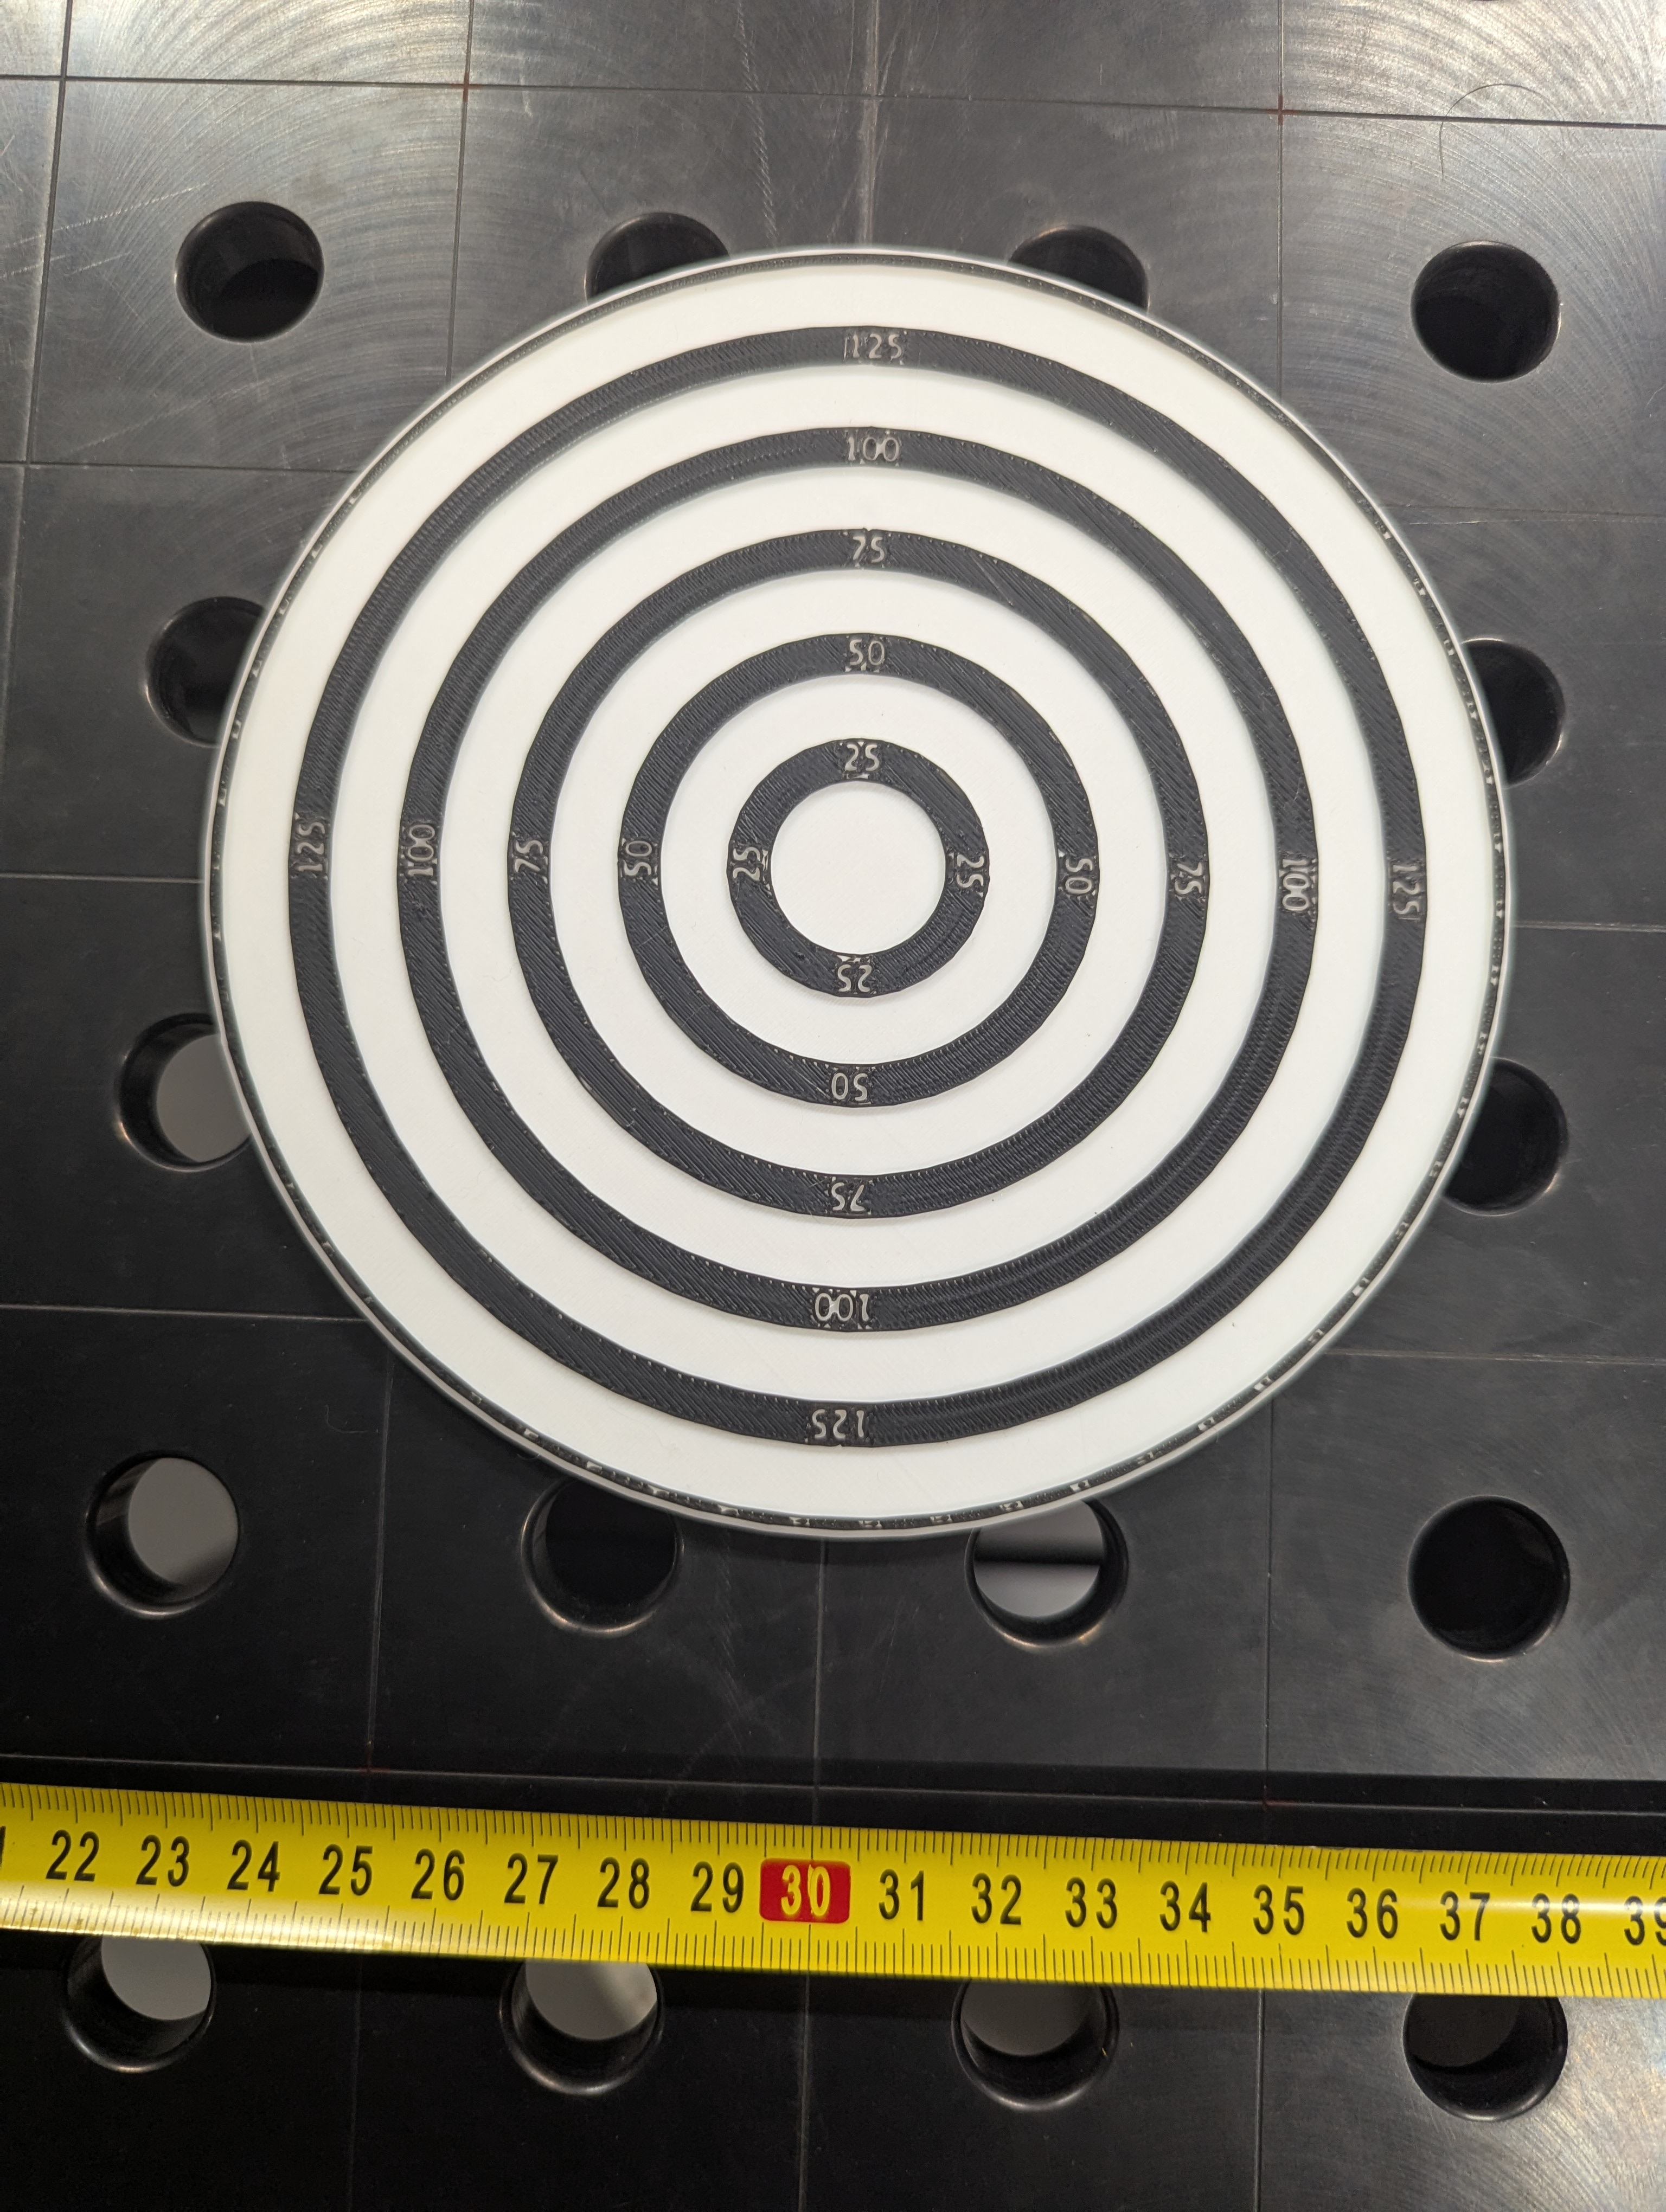
\includegraphics[width=\linewidth]{figures/precisionTest/shootingDiscX.jpg}
    \caption*{X direction of disc}
\end{minipage}
\hfill
\begin{minipage}{0.48\textwidth}
    \centering
    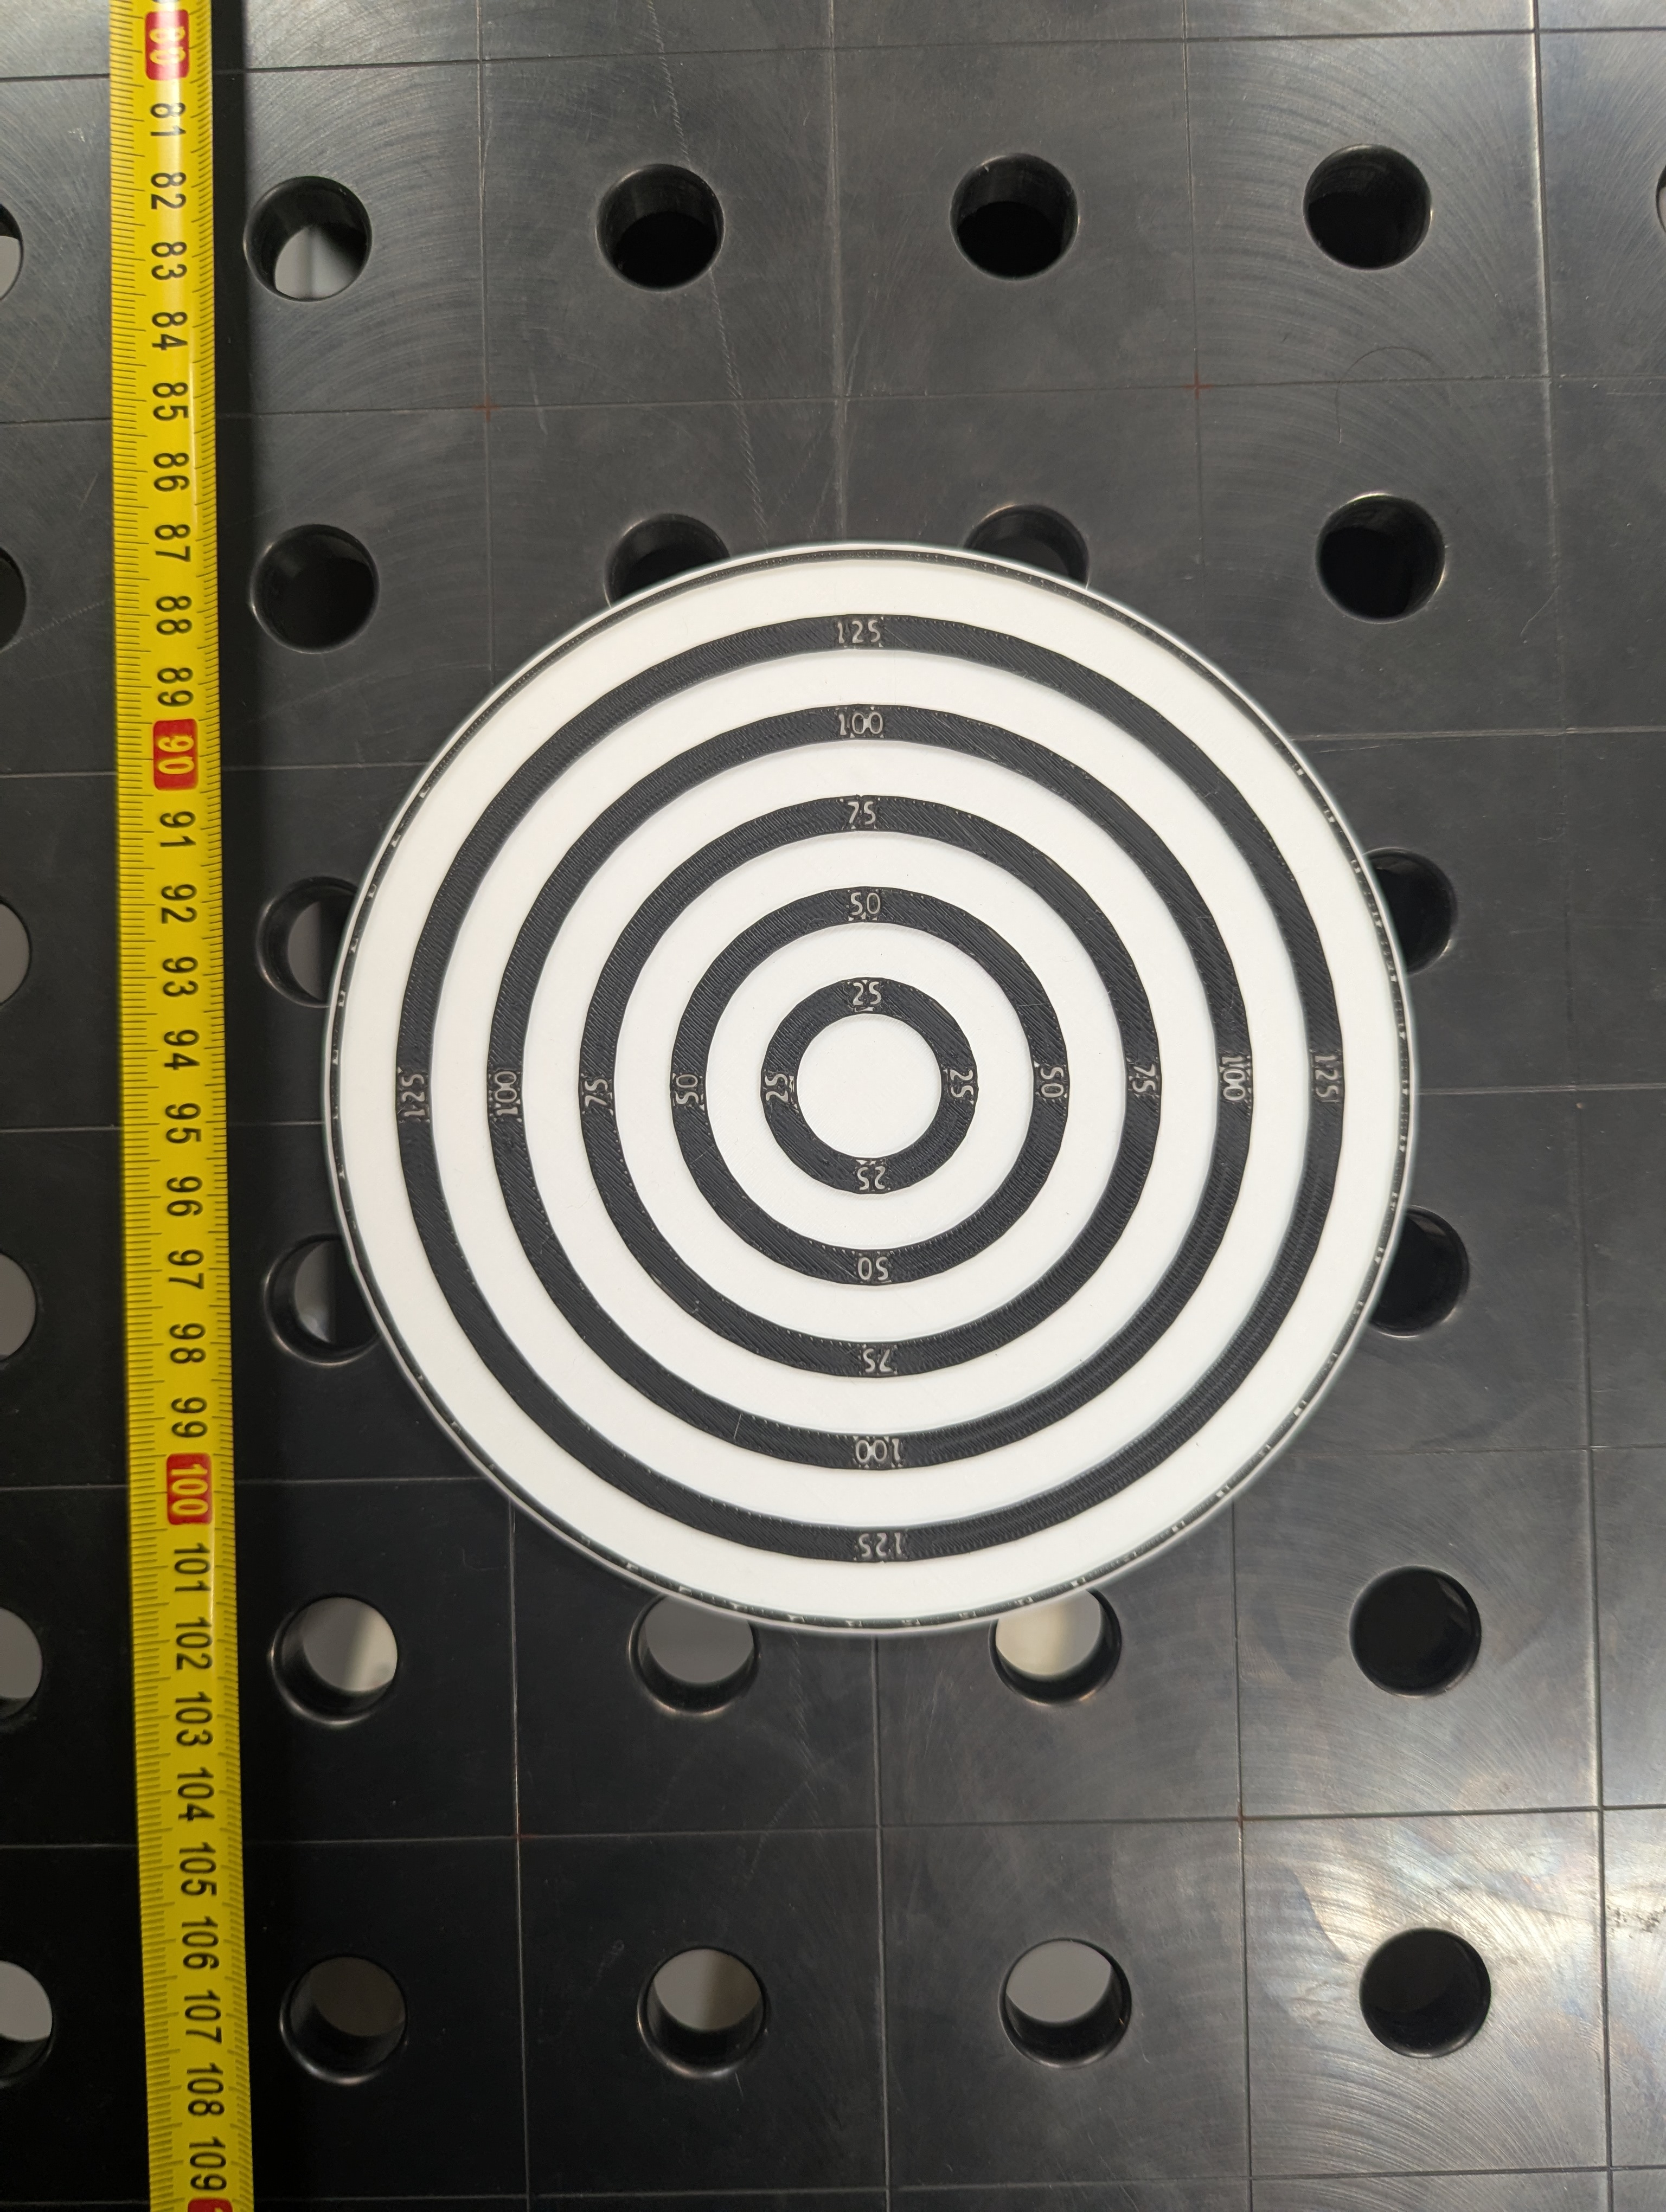
\includegraphics[width=\linewidth]{figures/precisionTest/shootingDiscY.jpg}
    \caption*{Y direction of disc}
\end{minipage}
\end{figure}
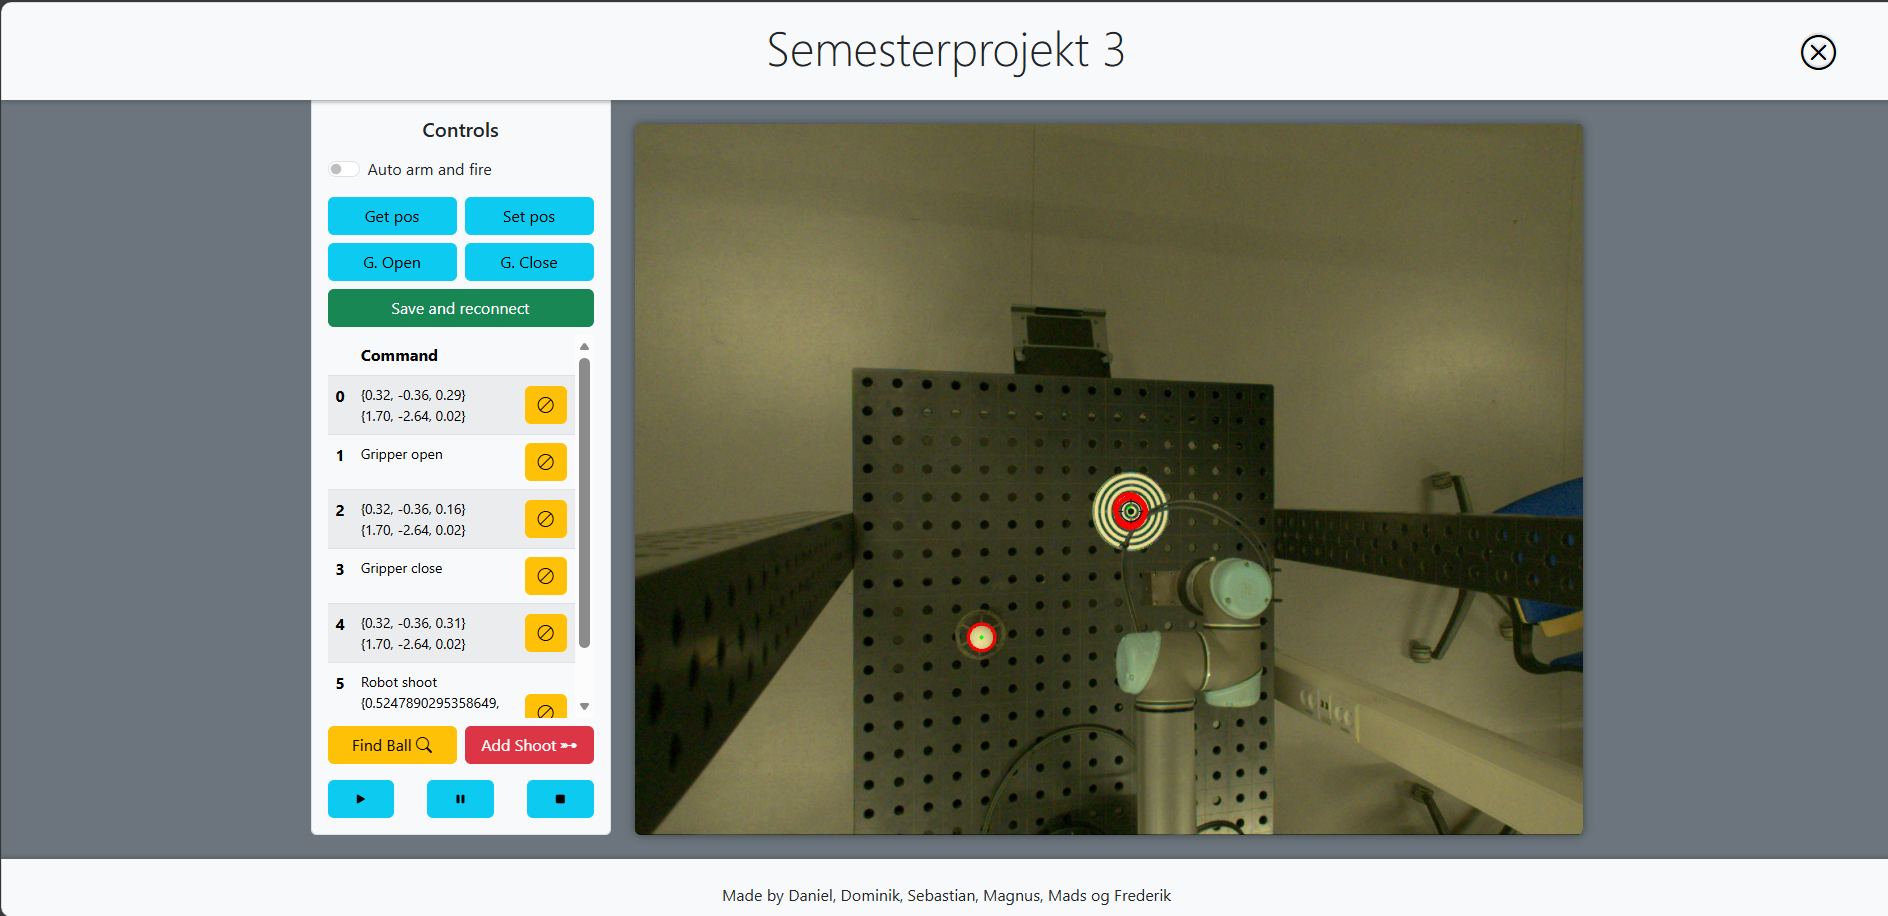
\includegraphics[width=100mm,center]{figures/precisionTest/screenShot.png}
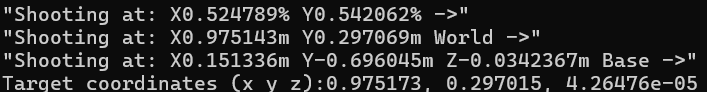
\includegraphics[width=190mm,center]{figures/precisionTest/testDetaljer.png}

As you can see, the x direction is a little off by 2,5cm in x+ direction, but the y direction is pretty much on point.

As it can be really hard to see how precise we hit, we have made a shooting disc. I will grade it with a inverted point system as to how good it hit it and if outside, i will grade it "out".

All the tests are videorecorded and can be found at "tests/servoJ\_VS\_speedJ precisionstest"

The disc is 150mm in diameter.

\subsubsection{servoJ precision}
\begin{tabular}{|c|c|}
\hline
test & result(mm) \\ \hline
1 & out \\ \hline
2 & out \\ \hline
3 & out \\ \hline
4 & 75 \\ \hline
5 & 50 \\ \hline
6 & 0 \\ \hline
7 & out \\ \hline
8 & out \\ \hline
9 & 50 \\ \hline
10 & 12.5 \\ \hline
11 & 50 \\ \hline
12 & 0 \\ \hline
13 & 50 \\ \hline

\end{tabular}

We hit the disc 8/13 times.\newline
The precision when it did hit the disc was about 36mm in radius which is much more precise than expected. 

\subsubsection{speedJ precision}

Here precision output has also been posted in corresponding folders

I will fail the test if we hit protective stop and call it PS which is also out.

\begin{tabular}{|c|c|}
\hline
test & result(mm) \\ \hline
1 & PS \\ \hline
2 & PS \\ \hline
3 & out \\ \hline
4 & 25 \\ \hline
5 & out \\ \hline
6 & out \\ \hline
7 & PS \\ \hline

\end{tabular}

We hit the disc 1/7 times.\newline
Also we hit protective stop 3/7 times.\newline
The precision when it did hit the disc was unusable. 

\subsection{Gripper response speed test} %kan godt være denne del skal flyttes til robotControl efter sektionen nu hedder evaluation og ikke tests
To ensure accuracy of our throw, it's important that we both release the ball while the robot is moving and at the correct position. This test will be focusing on the latter.
As out robot receives new positions to go to at a very quick speed (8ms), we need to ensure that the latency when sending a command to the gripper to when the gripper starts moving doesn't make our gripper release the ball at the wrong position.

The TCP communication works by us sending a command to the gripper and the gripper sending back an acknowledgement that it received the command before moving. By sending the command and then Immediately starting a timer that stops when we receive the ACK response meaning the gripper acknowledges the command and starts moving.

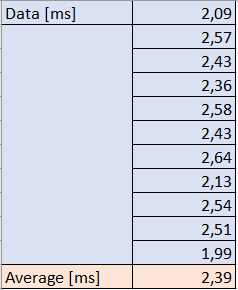
\includegraphics[width=50mm,center]{figures/GripData.PNG}
These are the 11 datapoints from said test. The average response time from the gripper to acknowledge the command is 2.39 ms which should result in no issues as to ensuring the ball is released at the correct time. If the ball is released exactly at the same time we receive the acknowledgement command, we can determine that the slight delay we get is irrelevant to the success of our throw.

However, what this test does not take into consideration is that just because we receive the confirmation that the gripper's fingers are moving, does not necessarily mean it immediately releases the ball at that exact time although it would seem like it from the naked eye. Ensuring this would require a much more extensive test. It is also possible that the gripper starts moving directly after it receives the command but before we receive the confirmation, reducing our delay time by perhaps half if it takes as much time to receive the confirmation as it did send the command.

\subsection{Final Product Testing}
To evaluate the final integrated product against the set goal, several tests were performed. The set goal was to hit the target 80  \% of all throws. The target counts as being hit, when the projectile lands within an orange 100 mm x 100 mm square box with a center point at the target position. 11 throws with varying target points were performed on this box and 3 out 11 throws were landed within the box. This gives a success rate of 27.27 \%. 

\

